%Version 3 December 2023
% See section 11 of the User Manual for version history
%
%%%%%%%%%%%%%%%%%%%%%%%%%%%%%%%%%%%%%%%%%%%%%%%%%%%%%%%%%%%%%%%%%%%%%%
%%                                                                 %%
%% Please do not use \input{...} to include other tex files.       %%
%% Submit your LaTeX manuscript as one .tex document.              %%
%%                                                                 %%
%% All additional figures and files should be attached             %%
%% separately and not embedded in the \TeX\ document itself.       %%
%%                                                                 %%
%%%%%%%%%%%%%%%%%%%%%%%%%%%%%%%%%%%%%%%%%%%%%%%%%%%%%%%%%%%%%%%%%%%%%

%%\documentclass[referee,sn-basic]{sn-jnl}% referee option is meant for double line spacing

%%=======================================================%%
%% to print line numbers in the margin use lineno option %%
%%=======================================================%%

%%\documentclass[lineno,sn-basic]{sn-jnl}% Basic Springer Nature Reference Style/Chemistry Reference Style

%%======================================================%%
%% to compile with pdflatex/xelatex use pdflatex option %%
%%======================================================%%

%%\documentclass[pdflatex,sn-basic]{sn-jnl}% Basic Springer Nature Reference Style/Chemistry Reference Style


%%Note: the following reference styles support Namedate and Numbered referencing. By default the style follows the most common style. To switch between the options you can add or remove “Numbered” in the optional parenthesis.
%%The option is available for: sn-basic.bst, sn-vancouver.bst, sn-chicago.bst%

%%\documentclass[pdflatex,sn-nature]{sn-jnl}% Style for submissions to Nature Portfolio journals
% \documentclass[pdflatex,sn-basic]{sn-jnl}% Basic Springer Nature Reference Style/Chemistry Reference Style
\documentclass[pdflatex,sn-mathphys-num]{sn-jnl}% Math and Physical Sciences Numbered Reference Style
% \documentclass[pdflatex,sn-mathphys-ay]{sn-jnl}% Math and Physical Sciences Author Year Reference Style
%%\documentclass[pdflatex,sn-aps]{sn-jnl}% American Physical Society (APS) Reference Style
%%\documentclass[pdflatex,sn-vancouver,Numbered]{sn-jnl}% Vancouver Reference Style
% \documentclass[pdflatex,sn-apa]{sn-jnl}% APA Reference Style
%%\documentclass[pdflatex,sn-chicago]{sn-jnl}% Chicago-based Humanities Reference Style

%%%% Standard Packages
%%<additional latex packages if required can be included here>

\usepackage{graphicx}%
\usepackage{multirow}%
\usepackage{amsmath,amssymb,amsfonts}%
\usepackage{amsthm}%
\usepackage{mathrsfs}%
\usepackage[title]{appendix}%
\usepackage[table]{xcolor}%
\usepackage{textcomp}%
\usepackage{manyfoot}%
\usepackage{booktabs}%
% \usepackage{algorithm}%
% \usepackage{algorithmicx}%
% \usepackage{algpseudocode}%
\usepackage{listings}%
\usepackage{subcaption}

\usepackage{hyperref}
\usepackage[ruled,linesnumbered,vlined]{algorithm2e}
\usepackage{colonequals}
\usepackage{tikz}
\usetikzlibrary{positioning}
\usetikzlibrary{automata}

\tikzset{%
  zeroarrow/.style = {-stealth,dashed},
  onearrow/.style = {-stealth,solid},
  c/.style = {circle,draw,solid,minimum width=2em,
        minimum height=2em},
  r/.style = {rectangle,draw,solid,minimum width=2em,
        minimum height=2em}
}

%%%%

%%%%%=============================================================================%%%%
%%%%  Remarks: This template is provided to aid authors with the preparation
%%%%  of original research articles intended for submission to journals published
%%%%  by Springer Nature. The guidance has been prepared in partnership with
%%%%  production teams to conform to Springer Nature technical requirements.
%%%%  Editorial and presentation requirements differ among journal portfolios and
%%%%  research disciplines. You may find sections in this template are irrelevant
%%%%  to your work and are empowered to omit any such section if allowed by the
%%%%  journal you intend to submit to. The submission guidelines and policies
%%%%  of the journal take precedence. A detailed User Manual is available in the
%%%%  template package for technical guidance.
%%%%%=============================================================================%%%%

%% as per the requirement new theorem styles can be included as shown below
\theoremstyle{thmstyleone}%
\newtheorem{theorem}{Theorem}%  meant for continuous numbers
%%\newtheorem{theorem}{Theorem}[section]% meant for sectionwise numbers
%% optional argument [theorem] produces theorem numbering sequence instead of independent numbers for Proposition
\newtheorem{proposition}[theorem]{Proposition}%
%%\newtheorem{proposition}{Proposition}% to get separate numbers for theorem and proposition etc.

\theoremstyle{thmstyletwo}%
\newtheorem{example}{Example}%
\newtheorem{remark}{Remark}%

\theoremstyle{thmstylethree}%
\newtheorem{definition}{Definition}%

\raggedbottom
% \unnumbered% uncomment this for unnumbered level heads

\begin{document}

\title[Article Title]{Mona Reimplemented: WS1S Logic with Mata}

%%=============================================================%%
%% GivenName	-> \fnm{Joergen W.}
%% Particle	-> \spfx{van der} -> surname prefix
%% FamilyName	-> \sur{Ploeg}
%% Suffix	-> \sfx{IV}
%% \author*[1,2]{\fnm{Joergen W.} \spfx{van der} \sur{Ploeg}
%%  \sfx{IV}}\email{iauthor@gmail.com}
%%=============================================================%%

\author{\fnm{Michal} \sur{Šedý}}\email{xsedym02@stud.fit.vutbr.cz}

%%==================================%%
%%     Unstructured abstract        %%
%%==================================%%

\abstract{This paper focuses on the reimplementation of the decision procedure for WS1S logic, a second-order logic that can be decided using finite automata. The well known tool for WS1S logic decision, Mona, employs automata with transitions represented through binary decision diagrams (BDDs). Due to the integration of BDDs in automata operations, tasks like reversal cannot be executed in the conventional manner of reverting individual edges. Instead, the reversal of each BDD must be computed, potentially resulting in an exponential blowup. Motivated by these limitations, Pavel Bednar reimplemented Mona using a pure automata approach with the Mata library. This work optimizes the automata methodology, resulting in a significant speedup, up to ten times faster, in WS1S decision compared to Bednar's original reimplementation.}


\keywords{Finite Automata, Binary Decision Diagrams, WS1S, MONA, MATA}


\maketitle


%%==================================%%
%%          INTRODUCTION            %%
%%==================================%%

\section{Introduction}
    The most well-known decision procedures are SAT and SMT \cite{SAT_SMT}, which are widely used in various applications such as verification (e.g., predicate abstraction), test generation, hardware synthesis, minimization, artificial intelligence, etc. The SAT (satisfiability) problem is a decision problem that asks whether a given propositional formula is satisfiable. The SMT (satisfiability modulo theories) problem extends the SAT problem to the satisfiability of first-order formulas with equality and atoms from various first-order theories. There are various higher-order decision procedures such as WS1S, WS2S, WSkS, S1S, etc.

    This work focuses on WS1S, the weak monadic second-order theory of the first successor. The term "weak" refers to finite sets, "monadic" indicates unary relations, "second-order" allows the usage of quantifiers over the relations, and "first successor" means that there is only one successor (e.g., the structure is linear).  WS1S \cite{WS1S} has an extremely simple syntax and semantics: it is variation of predicate logic with first-order variable that denote natural numbers and second-order variables that denote finite sets of natural numbers, it has a single function symbol, which denotes the successor function and has usual comparison operators such as $\leq$, $=$, $\in$ and $\supseteq$. Richard Büchi presented approach how to decide WS1S using finite automata in \cite{Buchi} The main idea is to recursively transform each subformula of the main WS1S formula into deterministic finite automata (DFA) representing feasible interpretations and simulate boolean operations via the automata operations.

    The most commonly used tool for deciding WS1S and WS2S is Mona\footnote{accessible at \url{https://www.brics.dk/mona/index.html}}, which employs Büchi's recursion approach for the construction of finite automata with binary decision diagrams (BDD) to represent all automaton transitions. The use of BDD makes the decision faster, but at the cost of making some automata operations, such as reversion, expensive (potentially resulting in exponential blowup). Despite this limitation, Mona is widely utilized in various fields of program verification, including the verification of programs with complex dynamic data structures \cite{DDS1, DDS2}, string analysis \cite{string_analysis}, parametrized systems \cite{parametrized_systems}, distributed systems \cite{distributed_systems}, automatic synthesis \cite{automatic_synthesis}, hardware verification \cite{hardware_verification}, and many others.

    The previously mentioned problem with hard-to-compute automata operations when using BDDs motivated Bc. Pavel Bednář's master's thesis \cite{Bednar}. He reimplemented Mona's decision of WS1S by using a pure automata-based approach with the Mata automata library\footnote{available at: \url{https://github.com/VeriFIT/mata}}. The special type of edge, the \textit{jumping edge} has been introduced. The jumping edge contains information about how many variables can be jumped over. The primary idea behind introducing the jumping edge was to enable jumps not only over inner states but also over automaton states, with no upper limit on the maximal jump. However, despite this innovation, the jumping edge did not yield significant improvements in terms of space or time compression. Furthermore, it appears that jumping edges led to an overcomplication of algorithms.

    In our approach, we reimplemented Bednář's solution by enhancing each automaton state with an index corresponding to the variable ID, mirroring the indexing strategy used for each inner node in the ordered BDD employed by Mona. This index information allows us to determine the length of a jump based on the indices of the source and destination states in the automaton's transition. Due to the indexing sequence on states follows a pattern of $0, 1, \dots, n-1, 0, 1, \dots, n-1, 0, \dots$, the longest jump can only reach to the next state with an index of $0$. While this might appear to be a step backward from Bednář's approach, the limitation on the jump length simplifies all algorithms. Surprisingly, it results in a significantly faster decision of the input formula, up to 10 times faster, compared to the variant with jumping edges.

    The first section introduces basic notations, definition of finite automata, binary decision diagrams, and WS1S. In the second section, we delve into the background of automata construction from WS1S formulas. The third section provides a detailed description of algorithms for intersection, union, complement, determinization, and minimization of automata with indexes. Moving to the fourth section, we present a~comparison of decision times between the Mona tool, automata with jumping edges, and automata with indexes. The experiments are divided into two parts. Initially, automata operations are tested separately on the automata generated during Mona computation. Following that, the comparison is executed on the entire input formula.

%%==================================%%
%%          INTRODUCTION            %%
%%==================================%%

\section{Preliminaries}
    In this section, we briefly introduce the definitions of nondeterministic and deterministic automata, binary decision diagrams, and the WS1S logic.

    \subsection{Automata}

        \begin{definition}
            A deterministic finite automaton is a 5-tuple $M = (Q, \Sigma, \delta, q_0, F)$, where its components are:
            \begin{itemize}[noindent]
                \item $Q$ is a finite nonempty set of states,
                \item $\Sigma$ is an alphabet,
                \item $\delta : Q \times \Sigma \rightarrow Q$ is a transition function,
                \item $q \in Q$ is an initial state, and
                \item $F \subseteq Q$ is a set of final states.
            \end{itemize}
        \end{definition}

        \begin{definition}
            A nondeterministic finite automaton is a 5-tuple $M = (Q, \Sigma, \delta, Q_0, F)$, where $Q$, $\Sigma$, and $F$ are defined identically as for the DFA. The transition function $\delta$~is defined as $\delta : Q \times \Sigma \rightarrow 2^{Q}$ and $Q_0 \subseteq Q$ is a nonempty set of initial states.
        \end{definition}

        Nondeterminism allows the automaton to make transitions to more than one successor based on the current state and the read input symbol. In contrast, its deterministic variant can transition to at most one state. Nondeterminism keeps the automaton more compact, but certain operations such as complementation cannot be performed directly on NFA. Therefore determinization is required beforehand.

    \subsection{Binary Decision Diagrams}
        Representation of the boolean function $\phi$ with $n$ logical variables leads to $2^n$ transitions for each automaton state in order to cover every possible combination of logical values. This exponential number of transitions can be reduced using Binary Decision Diagrams (BDDs). Binary Decision Diagrams provide a compact and, most importantly, canonical representation for logical functions in the form $\phi: \{0, 1\}^* \rightarrow \{0, 1\}$.

        \vspace*{0.5em}

        \begin{definition}
            The binary decision diagram \cite{BDD} is rooted, directed, connected, and acyclic graph defined as a 7-tuple $G = (N, T, var, low, high, root, val)$ where:
            \begin{itemize}[noindent]
                \item $N$ is finite set on non-terminal (inner) nodes,
                \item $T$ is a finite set of terminal nodes (leaves) such that $N \cap T = \emptyset$,
                \item $var : N \rightarrow N \cup T$ defines the low and high successors of the inner nodes,
                \item $root \in N \cup T$ is the root node, and
                \item $val : T \rightarrow \{0, 1\}$ assignes logical value to the leaves.
            \end{itemize}
        \end{definition}

        The size of the BDD is not determined only by the number of logical variables used within the function $\phi$ but also by the ordering of the variables in the BDD. The best variable ordering can result in a BDD with a linear (in the number of variables) number of nodes, while the worst ordering can lead to an exponential size.

        \begin{figure}[h]
            \centering
            \begin{subfigure}{0.5\textwidth}
                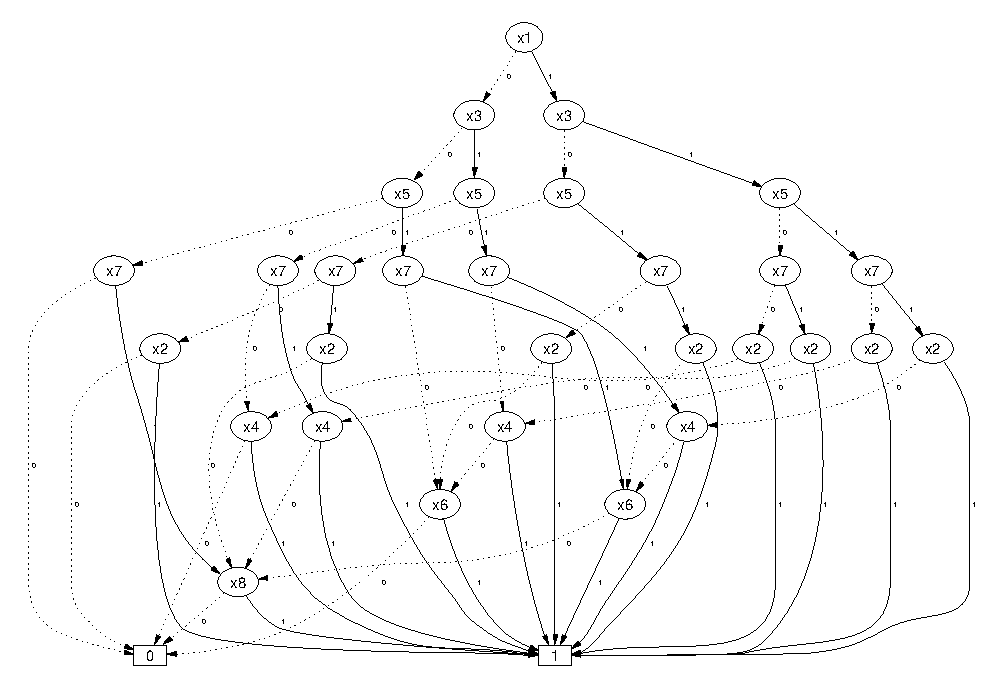
\includegraphics[width=1.2\textwidth]{Figures/BDD_Variable_Ordering_Bad.pdf}
            \end{subfigure}
            \hspace*{2cm}
            \begin{subfigure}{0.3\textwidth}
                \hspace*{1cm}
                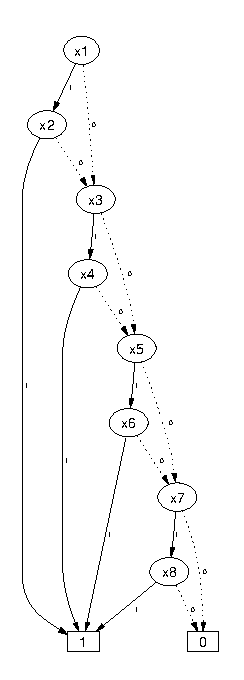
\includegraphics[width=0.5\textwidth]{Figures/BDD_Variable_Ordering_Good.pdf}
            \end{subfigure}
            \caption{Two bdds for the function $f(x1,\dots, x_{2n}) = x_1x_2 + x_3x_4 + \cdots, x_{2n-1}x_{2n}$ with bad variable ordering (on the left) and good variable ordering (on the right).}
            \label{figure::ordering}
        \end{figure}

        Consider the Boolean function $f(x_1, \dots, x_{2n}) = x_1x_2 + x_3x_4 + \cdots + x_{2n-1}x_{2n}$. Using the variable ordering $x_1 < x_3 < \cdots < x_{2n-1} < x_2 < x_4 < \cdots < x_{2n}$, the Binary Decision Diagram (BDD) requires $2^{n+1}$ nodes to represent the function. Using the ordering $x_1 < x_2 < x_3 < x_4 < \cdots < x_{2n-1} < x_{2n}$, the BDD consists of $2n + 2$ nodes. An example of such orderings is shown in Figure \ref{figure::ordering}. The problem of finding the best variable ordering is NP-hard \cite{BDD_np-hard}. However, various heuristics exist to address this challenge \cite{BDD_heuristics}.

        \vspace*{0.5em}

        \begin{definition}
            Let $\prec$ be a given ordering on logical variables $Var$, a Binary Decision Diagram (BDD) $G$ is ordered (OBDD) with respect to $\prec$ if, for every $n \in \mathbb{N}$, the following conditions hold:
            \begin{enumerate}[noindent]
                \item $low(n) \in N \implies var(n) \prec var(low(n))$
                \item $high(n) \in N \implies var(n) \prec var(high(n))$
            \end{enumerate}
        \end{definition}

        \begin{definition}
            The OBDD $G = (N, T, var, low, high, root, val)$ is a Reduced OBDD (ROBDD) if the following conditions are satisfied:
            \begin{enumerate}[noindent]
                \item $\forall t_1, t_2 \in T : val(t_1) \neq val(t_2)$
                \item There are no isomorphic subgraphs in $G$
                \item $\forall n_1, n_2 \in N : low(n_1) \neq low(n_2) \lor high(n_1) \neq high(n_2)$
            \end{enumerate}
        \end{definition}

        \begin{figure}[h]
            \centering
            \begin{subfigure}{0.45\textwidth}
                \centering
                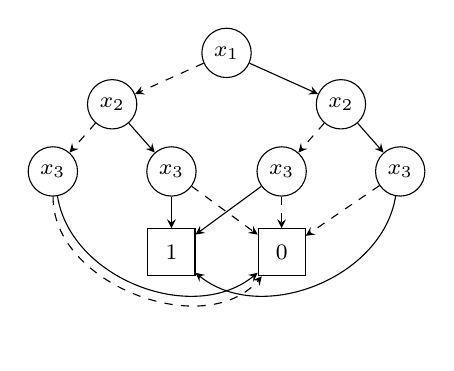
\begin{tikzpicture}[node distance=0.4cm and 0.3cm]\footnotesize
                    \node[c] (x1) {$x_1$};
                    \node[c] (x2a) [below left=0.2cm and 1cm of x1] {$x_2$};
                    \node[c] (x2b) [below right=0.2cm and 1cm of x1] {$x_2$};
                    \node[c] (x3a) [below left=of x2a] {$x_3$};
                    \node[c] (x3b) [below right=of x2a] {$x_3$};
                    \node[c] (x3c) [below left=of x2b] {$x_3$};
                    \node[c] (x3d) [below right=of x2b] {$x_3$};
                    \node[r] (one) [below=of x3b] {1};
                    \node[r] (zero) [below=of x3c] {0};

                    \draw[onearrow] (x1) -- (x2b);
                    \draw[onearrow] (x2a) -- (x3b);
                    \draw[onearrow] (x2b) -- (x3d);
                    \draw[onearrow] (x3a) to[bend right=60] (zero);
                    \draw[onearrow] (x3b) -- (one);
                    \draw[onearrow] (x3c) -- (one);
                    \draw[onearrow] (x3d) to[bend left=60] (one);

                    \draw[zeroarrow] (x1) -- (x2a);
                    \draw[zeroarrow] (x2a) -- (x3a);
                    \draw[zeroarrow] (x2b) -- (x3c);
                    \draw[zeroarrow] (x3a) to[bend right=70] (zero);
                    \draw[zeroarrow] (x3b) -- (zero);
                    \draw[zeroarrow] (x3c) -- (zero);
                    \draw[zeroarrow] (x3d) -- (zero);
                 \end{tikzpicture}
            \end{subfigure}
            \begin{subfigure}{0.25\textwidth}
                \centering
                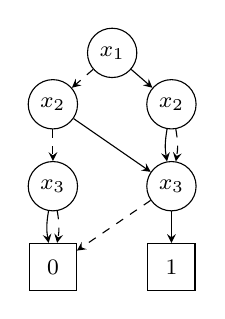
\begin{tikzpicture}[node distance=0.4cm and 0.3cm]\footnotesize
                    \node[c] (x1) {$x_1$};
                    \node[c] (x2a) [below left=0.2cm and 0.3cm of x1] {$x_2$};
                    \node[c] (x2b) [below right=0.2cm and 0.3cm of x1] {$x_2$};
                    \node[c] (x3a) [below=of x2a] {$x_3$};
                    \node[c] (x3b) [below=of x2b] {$x_3$};
                    \node[r] (one) [below=of x3b] {1};
                    \node[r] (zero) [below=of x3a] {0};

                    \draw[onearrow] (x1) -- (x2b);
                    \draw[onearrow] (x2a) -- (x3b);
                    \draw[onearrow] (x2b) to[bend right=10] (x3b);
                    \draw[onearrow] (x3a) to[bend right=10] (zero);
                    \draw[onearrow] (x3b) -- (one);

                    \draw[zeroarrow] (x1) -- (x2a);
                    \draw[zeroarrow] (x2a) -- (x3a);
                    \draw[zeroarrow] (x2b) to[bend left=10] (x3b);
                    \draw[zeroarrow] (x3a) to[bend left=10] (zero);
                    \draw[zeroarrow] (x3b) -- (zero);
                 \end{tikzpicture}
            \end{subfigure}
            \begin{subfigure}{0.25\textwidth}
                \centering
                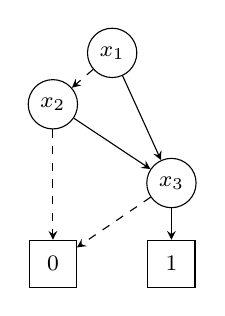
\begin{tikzpicture}[node distance=0.4cm and 0.3cm]\footnotesize
                    \node[c] (x1) {$x_1$};
                    \node[c] (x2) [below left=0.2cm and 0.3cm of x1] {$x_2$};
                    \node[c] (x3) [below right=1.2cm and 0.3cm of x1] {$x_3$};
                    \node[r] (one) [below=of x3] {1};
                    \node[r] (zero) [below= 1.4cm of x2] {0};

                    \draw[onearrow] (x1) -- (x3);
                    \draw[onearrow] (x2) -- (x3);
                    \draw[onearrow] (x3) -- (one);

                    \draw[zeroarrow] (x1) -- (x2);
                    \draw[zeroarrow] (x2) -- (zero);
                    \draw[zeroarrow] (x3) -- (zero);
                 \end{tikzpicture}
            \end{subfigure}
            \caption{From left to right, an OBDD satisfies the first, second, and third conditions as specified in the definition of ROBDD.}
        \end{figure}

        \vspace*{-1em}

        \begin{theorem}
            \label{theorem:ROBDD}
            For every Boolean function $\phi$ over some set of variables $Var$ and every variable ordering $\prec$ on $Var$, there is a unique (up to isomorphism) reduced OBDD (with respect to $\prec$) $G_\phi$ which represents $\phi$. \cite{BDD}"
        \end{theorem}

        \vspace*{0.5em}

        Based on Theorem \ref{theorem:ROBDD}, checking the equivalence of two functions, $\phi_1$ and $\phi_2$, represented by Reduced OBDDs (ROBDDs) $G_1$ and $G_2$ is equivalent to checking the isomorphism of $G_1$ and $G_2$.

        Moreover, if several Boolean functions are represented with one shared ROBDD with multiple roots, as Mona does, the equivalence checking is reduced from isomorphism checking to simply checking the identity of the BDD roots.


    \subsection{WS1S}
        Richard Büchi showed that WS1S is equivalent to regular expressions and can therefore be represented by finite automata \cite{Buchi}. In this subsection, the simplification of the WS1S formula and its semantics will be presented, followed by the transformation of atomic formulae to automata. The main source for this subsection was \cite{Mona_manual}.

        \subsubsection*{Formula simplification}
            First-order terms are encoded as second-order terms since a first-order value can be seen as a singleton second-order value. Also, booleans can be encoded using the first position in the input automaton string.

            All second-order terms are 'flattened' by introducing new variables that contain the values of all subterms. For example, the formula $A = (B \cup C) \cap D$ will be transformed into the form $\exists V : A = V \cap D \land V = B \cup C$, where $V$ is a new variable.

            Subformulae are simplified to contain fewer operators. As a result, only basic operations have to be implemented by the solver. The abstract syntax for simplified WS1S formulas can be defined by the following grammar:
            $$
                \phi \colonequals \neg \phi' | \phi' \land \phi'' | \exists P_i : \phi' | P_i \subseteq P_j | P_i = P_j \setminus P_k | P_i = P_j + 1
            $$

        \subsubsection*{Semantic}
            Given the main formula $\phi_0$, we define its semantic inductively relative to a string $w$ over the alphabet $\mathbb{B}^k$, where $\mathbb{B} = {0, 1}$ and $k$ is the number of variables in $\phi_0$. Assume every variable of $\phi_0$ is assigned a unique number in the range $1, 2, \dots, k$, called the \textit{variable index}. The string $w$ now determines an interpretation $w(P_i)$ of $P_i$, defined as the finite set ${j ,|, \text{the } j\text{th bit in the } P_i\text{-track is 1}}$. For example, the formula $\phi_0 \equiv \exists C : A = B \setminus C$ has variables $A$, $B$, and $C$, which are assigned the indices 1, 2, and 3, respectively. A typical string $w$ over $\mathbb{B}^3$ looks like:

            $$
            \begin{matrix}
                A\\
                B\\
                C
            \end{matrix}
            \hspace*{2em}
            \begin{pmatrix}
                1\\
                0\\
                1
            \end{pmatrix}
            \begin{pmatrix}
                0\\
                0\\
                1
            \end{pmatrix}
            \begin{pmatrix}
                1\\
                1\\
                0
            \end{pmatrix}
            \begin{pmatrix}
                0\\
                0\\
                0\\
            \end{pmatrix}
            $$

            \vspace*{0.5em}

            \noindent It's important to note that $w$ with the suffix $(0^*)^T$ defines the same interpretation as $w$. Therefore, the minimum $w$ is such a string that there is no such non-empty suffix. The semantics of a formula $\phi$ is defined inductively:
                \begin{alignat*}{2}
                    &w \vDash \neg \phi' \quad && \textnormal{iff}\quad  w \nvDash \phi'\\
                    &w \vDash \phi' \land \phi'' \quad &&\textnormal{iff}\quad  w \vDash \phi' \land w \vDash \phi''\\
                    &w \vDash \exists P_i : \phi' \quad &&\textnormal{iff}\quad  \exists finite(M) \subseteq \mathbb{N} : w[P_i \mapsto M] \vDash \phi'\\
                    &w \vDash P_i \subseteq P_j \quad &&\textnormal{iff}\quad  w(P_i) \subseteq w(P_j)\\
                    &w \vDash P_i = P_j \setminus P_k \quad &&\textnormal{iff}\quad  w(P_i) = w(P_j) \setminus w(P_k)\\
                    &w \vDash P_i = P_j + 1 \quad &&\textnormal{iff}\quad  w(P_i) = \{j + 1\,|\, j \in w(P_j)\}
                \end{alignat*}

                where we use the notation $w[P_i \mapsto M]$ for the shortest string $w'$ that interprets all variables $P_j$, $j \neq i$, as $w$ does but interprets $P_i$ as $M$. Note that if we assume that $w$ is minimum, then $w'$ decomposes into $w' = w \cdot w''$, where $w''$ is a string of letters of the form $(0^*X0^*)^T$, and the $i$th component is the only one that may be different from 0.

        \subsubsection*{Automaton construction}
            The input formula $\phi$ is recursively transformed into the deterministic finite automaton that represents the set of satisfying strings $L(\phi) = {w,|, w \vDash \phi}$. The translation of atomic and composite formulae to deterministic finite automata follows:


            \vspace*{0.5em}

            \begin{itemize}
                \item $\phi = P_1 \subseteq P_2$:
                    \begin{figure}[h]
                        \centering
                        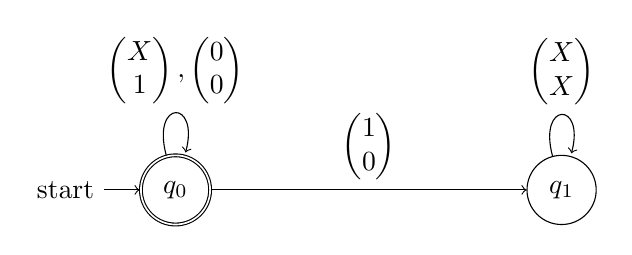
\begin{tikzpicture}
                            \centering
                            \node[state, initial, accepting] (q0) {$q_0$};
                            \node[state] (q1) [right=4cm of q0]{$q_1$};

                            \path[->] (q0) edge node[above] {$\begin{pmatrix}1\\0\end{pmatrix}$} (q1)
                                    (q0) edge[loop above] node {$\begin{pmatrix}X\\1\end{pmatrix},\begin{pmatrix}0\\0\end{pmatrix}$} ()
                                    (q1) edge[loop above] node {$\begin{pmatrix}X\\X\end{pmatrix}$} ();
                        \end{tikzpicture}
                    \end{figure}
                \vspace*{0.5em}
                \item $\phi = P_1 = P_2 \setminus P_3$:
                    \begin{figure}[h]
                        \centering
                        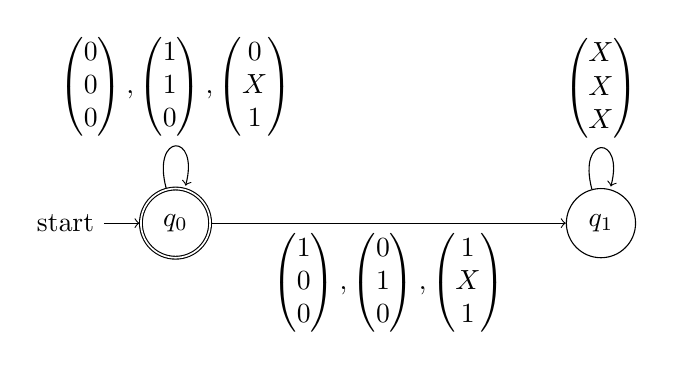
\begin{tikzpicture}
                            \centering
                            \node[state, initial, accepting] (q0) {$q_0$};
                            \node[state] (q1) [right=4.5cm of q0]{$q_1$};

                            \path[->] (q0) edge node[below] {$\begin{pmatrix}1\\0\\0\end{pmatrix},\begin{pmatrix}0\\1\\0\end{pmatrix},\begin{pmatrix}1\\X\\1\end{pmatrix}$} (q1)
                                    (q0) edge[loop above] node {$\begin{pmatrix}0\\0\\0\end{pmatrix},\begin{pmatrix}1\\1\\0\end{pmatrix},\begin{pmatrix}0\\X\\1\end{pmatrix}$} ()
                                    (q1) edge[loop above] node {$\begin{pmatrix}X\\X\\X\end{pmatrix}$} ();
                        \end{tikzpicture}
                    \end{figure}
                \newpage
                \item $\phi = P_1 = P_2 + 1$:
                    \vspace*{-1em}
                    \begin{figure}[h]
                        \centering
                        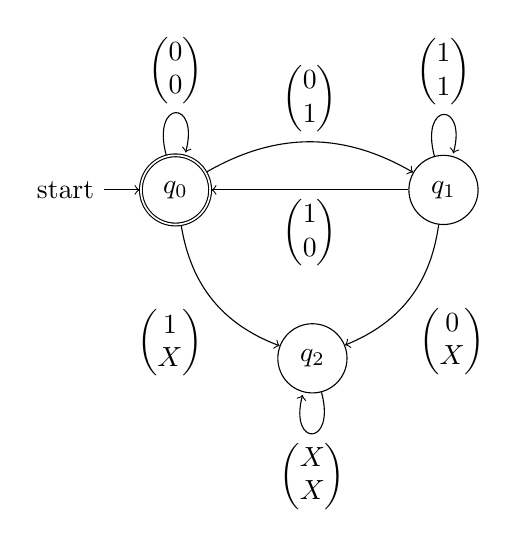
\begin{tikzpicture}
                            \centering
                            \node[state, initial, accepting] (q0) {$q_0$};
                            \node[state] (q1) [right=2.5cm of q0]{$q_1$};
                            \node[state] (q2) [below right=1.5cm and 1.1cm of q0] {$q_2$};
                            \path[->] (q0) edge[bend left] node[above] {$\begin{pmatrix}0\\1\end{pmatrix}$} (q1)
                                      (q0) edge[loop above] node[above] {$\begin{pmatrix}0\\0\end{pmatrix}$} ()
                                      (q0) edge[bend right] node[below left] {$\begin{pmatrix}1\\X\end{pmatrix}$} (q2)
                                      (q1) edge[bend left] node[below right] {$\begin{pmatrix}0\\X\end{pmatrix}$} (q2)
                                      (q1) edge node[below] {$\begin{pmatrix}1\\0\end{pmatrix}$} (q0)
                                      (q1) edge[loop above] node[above] {$\begin{pmatrix}1\\1\end{pmatrix}$} ()
                                      (q2) edge[loop below] node[below] {$\begin{pmatrix}X\\X\end{pmatrix}$} ();
                        \end{tikzpicture}
                    \end{figure}
                \item $\phi = \neg \phi'$: Negation of a formula corresponds to automaton complementation. If we have already calculated $A'$ such that $L(\phi') = L(A')$, then $L(\neg \phi') = \complement L(\phi') = \complement L(A') = L(\complement A')$, where $\complement$ denotes both language complementation and automata complementation. If the automaton is complete and deterministic, then complementation can be done by swapping accepting and non-accepting states.
                \vspace*{0.5em}
                \item $\phi = \phi' \land \phi''$: Conjunction corresponds to language intersection, $L(\phi' \land \phi'') = L(\phi') \cap L(\phi'')$. So, the resulting automaton $A$ is obtained by the production of automata $A' \times A''$, where $L(\phi') = L(A')$ and $L(\phi'') = L(A'')$.
                \vspace*{0.5em}
                \item $\phi = \exists P_i : \phi'$:  Intuitively, the desired automaton $A$ acts as the automaton $A'$ for $\phi'$ except that it is allowed to guess the bits on the $P_i$-track. The resulting automaton $A$ is nondeterministic. It is necessary to apply determinization and adjust the automaton $A$ in such a way that each $w \in L(A)$ is minimal.
            \end{itemize}



\section{Automata representation}
    This section presents three different approaches on how to incorporate BDDs into finite automata. First, Mona's approach using shared BDDs is shown, followed by approaches that utilize jumping edges or state indexing.

    \subsection{Mona}
        Mona represents the transition function not only using a single BDD (as in the case of Kripke structures) but with a \textit{shared multi-terminal }BDD (SMTBDD). The main difference from standard BDDs is that the leaves of SMTBDD do not contain boolean values 0 or 1 but rather states of the automaton.

        \vspace*{0.5em}

        \begin{definition}
            Let $M = (Q, \Sigma, \delta, q_0, F)$ be DFA. The SMTBDD is defined as a 7-tuple $G = (N, T, var, low, high, R, val)$ where:
            \begin{itemize}[noindent]
                \item $N$ is finite set on non-terminal (inner) nodes,
                \item $T$ is a finite set of terminal nodes (leaves) such that $N \cap T = \emptyset$,
                \item $var : N \rightarrow N \cup T$ defines the low and high successors of the inner nodes,
                \item $R \subseteq N \cup T$ is nonempty set of rules, and
                \item $val : T \rightarrow Q$ assignes states to the leaves.
            \end{itemize}
        \end{definition}

        For example, let the formula $\phi \equiv \exists p, q : p \neq q \land p \in X \cap Y \land q \ \in X \cap Y$ be represented by the automaton $M$ in Figure \ref{fig:mona}, where each state $r$, $s$, and $t$ contains information about whether it is accepting or not and points to its root node in the SMTBDD describing its transition relation. The data structure also contains a pointer to the initial state.

        \begin{figure}[h]
            \centering
            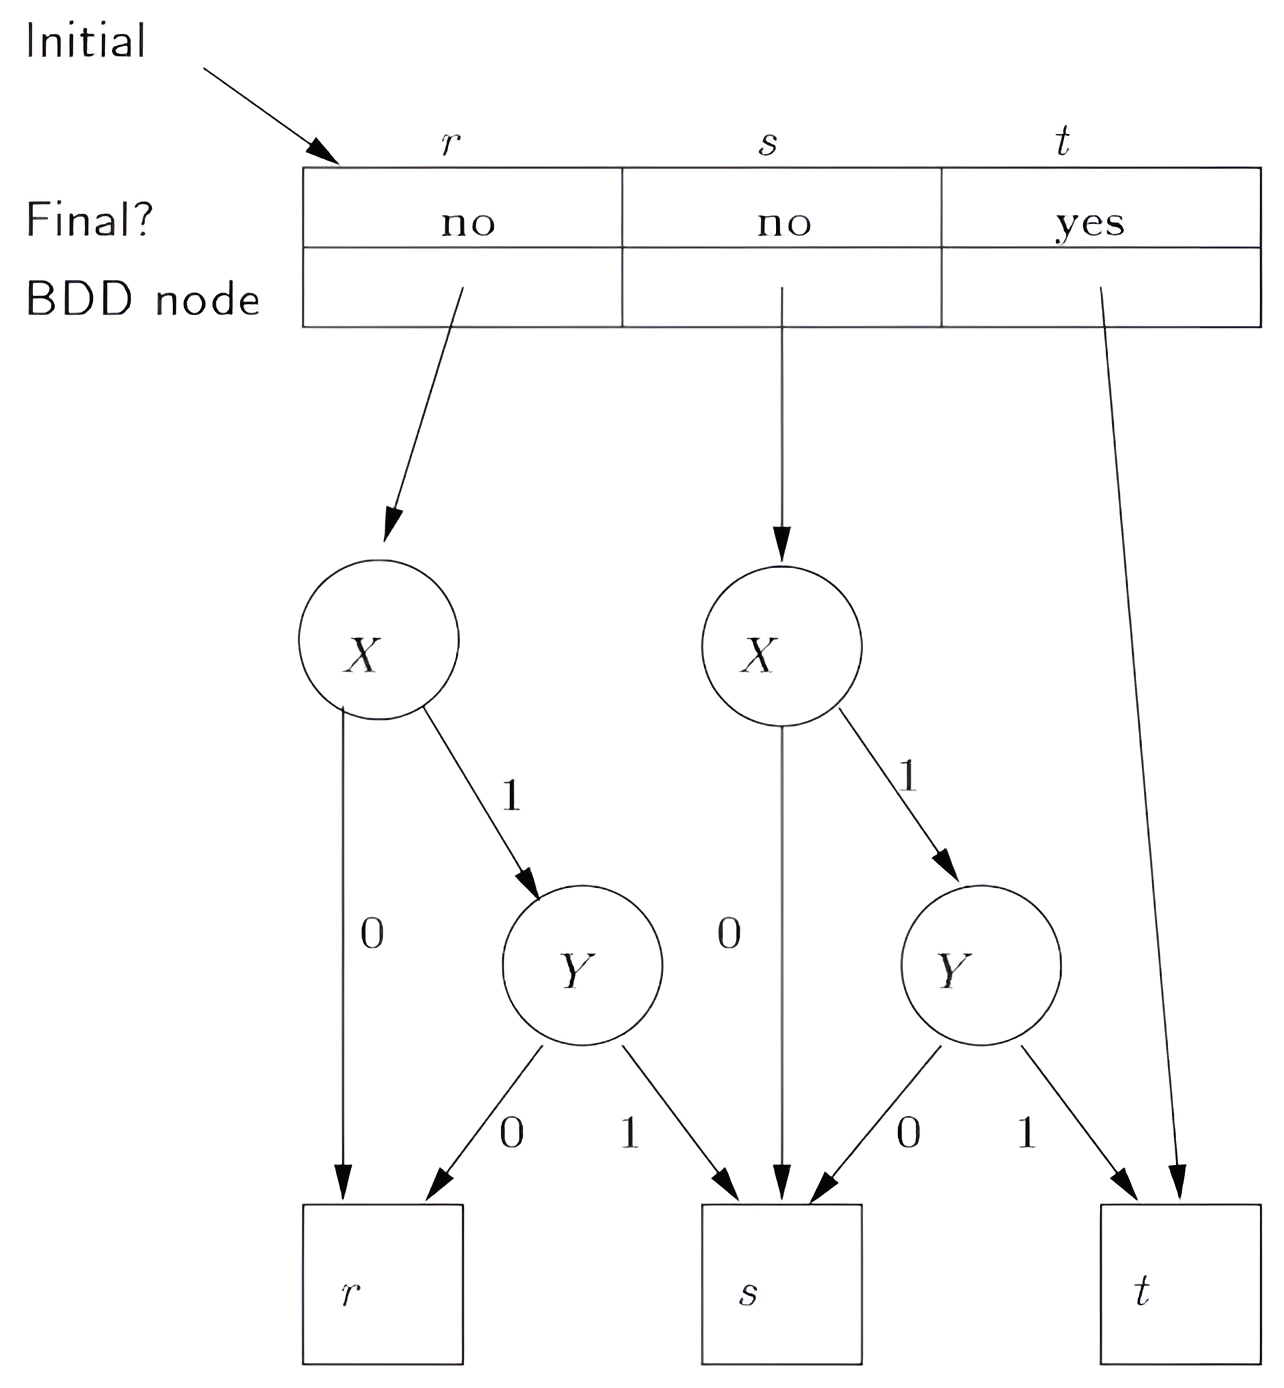
\includegraphics[width=0.5\textwidth]{Figures/mona_aut.png}
            \vspace*{0.5em}
            \caption{Mona automaton for the formula $\phi \equiv \exists p, q : p \neq q \land p \in X \cap Y \land q \ \in X \cap Y$.}
            \label{fig:mona}
        \end{figure}

        \vspace*{-2em}

    \subsection{Automata with Skip Edges}
        The main idea of Bednář's skip edges \cite{Bednar} is to integrate BDD nodes directly into the transitions of the automaton. This can be easily noted, as BDD has an automata-like structure. To simulate the functionality of a BDD, where each node has an assigned variable, it is necessary to use skip edges.

        \vspace*{0.5em}

        \begin{definition}
            Let $M = (Q, \Sigma, \delta, Q_0, F)$ be an NFA, then automaton with skip edges $N = (Q, \Sigma, \delta', Q_0, F)$ has transition function defined as $\delta' : Q \times \Sigma \rightarrow 2^{\mathbb{N} \times Q}$.
        \end{definition}

        \vspace*{0.5em}

        The transition function in the automaton with skip edges provides information about target states and the number of variables that have been jumped over. The skip edge with a length of 1 is a special case that has the same functionality as edges in NFA. $(n, r) \in \delta'(q, a)$ denotes that the automaton can move from state $q$ to $r$ after reading a symbol $a$ and then jump over $n-1$ variables.

        \vspace*{-1em}

        \begin{figure}[h]
            \centering
            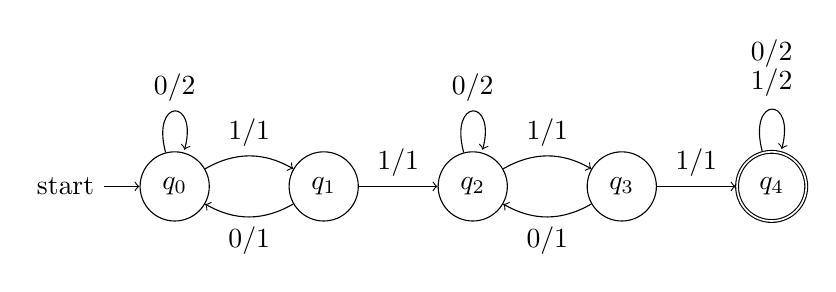
\begin{tikzpicture}
                \node[state, initial] (q0) {$q_0$};
                \node[state] (q1) [right=of q0]{$q_1$};
                \node[state] (q2) [right=of q1]{$q_2$};
                \node[state] (q3) [right=of q2]{$q_3$};
                \node[state, accepting] (q4) [right=of q3] {$q_4$};

                \path[->] (q0) edge[bend left] node[above] {$1/1$} (q1)
                          (q0) edge[loop above] node[above] {$0/2$} ()
                          (q1) edge[bend left] node[below] {$0/1$} (q0)
                          (q1) edge node[above] {$1/1$} (q2)
                          (q2) edge[bend left] node[above] {$1/1$} (q3)
                          (q2) edge[loop above] node[above] {$0/2$} ()
                          (q3) edge[bend left] node[below] {$0/1$} (q2)
                          (q3) edge node[above] {$1/1$} (q4)
                          (q4) edge[loop above] node[above] {$\begin{aligned}0/2\\[-1.5mm]1/2\end{aligned}$} ();
            \end{tikzpicture}
            \caption{An automaton with skip edges representing the language from Figure \ref{fig:mona}. A skip edge labeled with $a/n$ can be interpreted as a transition of length $n$ reading symbol $a$.}
        \end{figure}

        \vspace*{-1.5em}

        The potential benefit of skip edges is derived from the fact that the length of the jump edge is not limited. Therefore, the jump edge can traverse over many BDDs and automaton states. The demonstration of this benefit is shown in Figure \ref{fig:skip_edges}. However, it has to be mentioned that this approach overcomplicated algorithms and did not show improvement in space or time.

        \vspace*{-1.25em}

        \begin{figure}[h]
            \centering
            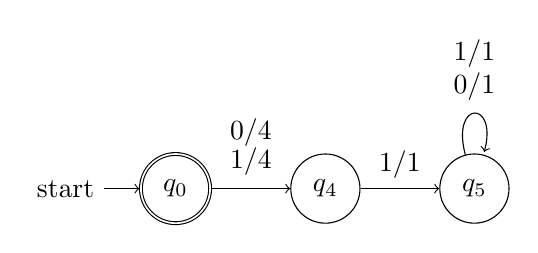
\begin{tikzpicture}
                \node[state, initial, accepting] (q0) {$q_0$};
                \node[state] (q4) [right=of q0]{$q_4$};
                \node[state] (q5) [right=of q4] {$q_5$};
                \path[->] (q0) edge node[above] {$\begin{aligned}0/4\\[-1.5mm]1/4\end{aligned}$} (q4)
                          (q4) edge node[above] {$1/1$} (q5)
                          (q5) edge[loop above] node[above] {$\begin{aligned}1/1\\[-1mm]0/1\end{aligned}$} ();
            \end{tikzpicture}
            \caption{Automaton with skip edges and a variable $X$ representing formula $3 \in X$.}
            \label{fig:skip_edges}
        \end{figure}

    \vspace*{2em}

    \subsection{Automata with Indexed States}
        The approach of an automaton with indexed states has been the main focus of the reimplementation. This automaton integrates BDDs directly while maintaining the indexes on its nodes (automaton states).

        \vspace*{0.5em}

        \begin{definition}
            Let $M = (Q, \Sigma, \delta, Q_0, F)$ be an NFA. The automaton $M$ is called an automaton with indexing if there exists an index function $\iota : Q \rightarrow \mathbb{N}_0$ such that the following conditions hold:
            \begin{enumerate}[noindent]
                \item $\forall q \in Q_0 : \iota(q) = 0$
                \item $\forall q \in F : \iota(q) = 0$
                \item $\forall q, r \in Q : \nexists a \in \Sigma : r \in \delta(q, a) \land \iota(r) \neq 0 \land \iota(q) \geq \iota(r)$
            \end{enumerate}
        \end{definition}

        The first and second conditions reflect the fact that only roots or leaves in the BDD can be initial and final states, respectively. The third condition demands that the part of the automaton simulating the BDD must be acyclic, with the exception of the root nodes/states with index 0.

        The index information determines the length of a jump based on the indices of the source and destination states in the automaton's transition. Due to the indexing sequence following a pattern of $0, 1, \dots, n-1, 0, 1, \dots, n-1, 0, \dots$, the longest jump can only reach to the next state with an index of $0$. Although it might seem like a~step back from Bednář's method, the restriction on jump length actually simplifies all algorithms. Interestingly, this leads to a noticeably faster evaluation of the input formula, up to 10 times faster when compared to the version incorporating skip edges.

        \begin{figure}[h]
            \centering
            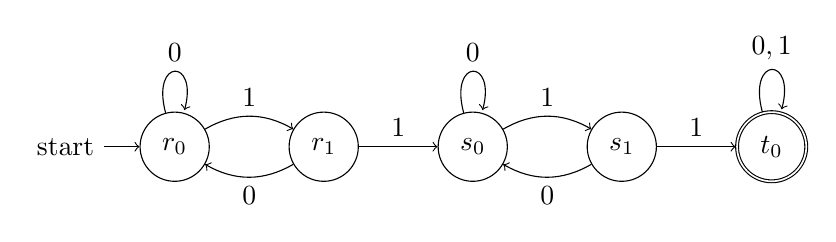
\begin{tikzpicture}
                \node[state, initial] (q0) {$r_0$};
                \node[state] (q1) [right=of q0]{$r_1$};
                \node[state] (q2) [right=of q1]{$s_0$};
                \node[state] (q3) [right=of q2]{$s_1$};
                \node[state, accepting] (q4) [right=of q3] {$t_0$};

                \path[->] (q0) edge[bend left] node[above] {$1$} (q1)
                          (q0) edge[loop above] node[above] {$0$} ()
                          (q1) edge[bend left] node[below] {$0$} (q0)
                          (q1) edge node[above] {$1$} (q2)
                          (q2) edge[bend left] node[above] {$1$} (q3)
                          (q2) edge[loop above] node[above] {$0$} ()
                          (q3) edge[bend left] node[below] {$0$} (q2)
                          (q3) edge node[above] {$1$} (q4)
                          (q4) edge[loop above] node[above] {$0,1$} ();
            \end{tikzpicture}
            \caption{Automaton with indexed states representing the language from Figure \ref{fig:mona}.}
        \end{figure}

\section{Automata operations}
    This section presents operations on automata with indexed states, which are utilized in the reimplementation of Mona using the Mata library. The primary concept of these operations is derived from Mata and modified to adapt state indexing.

    \subsection{Complement}
        The complementation method is the most straightforward approach for automata. It involves taking a complete deterministic automaton and swapping its accepting and nonaccepting states. Unlike classical complementation, only the accepting property of states with index $0$ is altered.

        \vspace*{0.5em}

        \begin{definition}
            Let $M = (Q, \Sigma, \delta, q_0, F)$ be a complete DFA with an index function $\iota : Q \rightarrow \mathbb{N}_0$. The complement of $M$ is defined as $\complement M = (Q, \Sigma, \delta, q_0, F')$, where:
            $$
            F' = \{q \in Q\,|\, \iota(q) = 0 \land q \notin F\}\setminus\{q_0\}
            $$
        \end{definition}

    \subsection{Intersection}
        The standard intersection algorithm generates the resulting automaton using product construction. It begins with the pair of initial states (one from each automaton) and moves synchronously to the pair of successors based on the transition symbol. The key idea is inspired by the \textit{Apply} method \cite{APPLY}, commonly used in Binary Decision Diagram (BDD) operations. In this adaptation of the standard intersection algorithm, the successor pair for the analyzed product pair is generated based on the state (or states in the case of identical indices) with the lower index. Meanwhile, the state with the higher index is duplicated.

        \begin{algorithm}
            \caption{An Intersection Algorithm}
            \small
            \DontPrintSemicolon
            \SetKwFunction{procA}{get_new_index}
            \SetKwFunction{procB}{create_state}
            \KwData{Two DFA $M = (Q_M, \Sigma_M, \delta_M, i_M, F_M)$ and $N = (Q_N, \Sigma_N, \delta_N, i_N, F_N)$ and tow index functions $\iota_M : Q_M \rightarrow \mathbb{N}_0$ and $\iota_N : Q_M \rightarrow \mathbb{N}_0$}
            \KwOut{Resulting DFA $A = (Q \subseteq Q_M \times Q_N, \Sigma \subseteq \Sigma_M \cup \Sigma_N, \delta, i, F) = M \cap N$ and index function $\iota Q \rightarrow \mathbb{N}_0$}

            \vspace*{0.5em}

            \SetKwProg{procA}{Procedure}{}{}
                \procA{\textnormal{Index($s_M$, $s_N$)}}{
                    \If{$\iota_N(s_N) = 0$}{
                        \Return{$\iota_M(s_M)$}\;
                    }\If{$\iota_M(s_M) = 0$}{
                        \Return{$\iota_N(s_N)$}\;
                    }
                    \Return{$min(\iota_M(s_M), \iota_N(s_N))$}\;
            }

            \vspace*{0.5em}

            \SetKwProg{procB}{Procedure}{}{}
                \procB{\textnormal{Createq\_State($x$, $y$)}}{
                    $worklist \leftarrow worklist \cup \{(x, y)\}$\;
                    $Q \leftarrow Q \cup \{(x, y)\}$\;
                    $\iota((x, y)) \leftarrow Index(x, y)$\;
                    \If{$x \in F_M \land y \in F_N$}{
                        $F \leftarrow F \cup (x, y)$\;
                    }
            }

            \vspace*{0.5em}

            $i \leftarrow (i_M, i_N)$\;
            $\iota(i) \leftarrow 0$\;
            $worklist \leftarrow \{i\}$\;
            $Q \leftarrow Q \cup \{i\}$\;
            \While{$worklist \neq \emptyset$}{
                $s \leftarrow worklist.pop()$\;
                $(s_M, s_N) \leftarrow s$\;
                \uIf{$\iota_M(s_M) = \iota_N(s_N)$}{
                    \ForAll{$a \in \Sigma_M \cap \Sigma_N : \delta_M(s_M, a) \in Q_M \land \delta_N(s_N, a) \in Q_N$}{
                        $\delta(s, a) \leftarrow (\delta_M(s_M, a), \delta_N(s_N, a))$\;
                        $Create\_State(\delta_M(s_M, a), \delta_N(s_N, a))$\;
                    }
                }\uElseIf{$(\iota_M(s_M) < \iota_N(s_N) \land \iota_M(s_M) \neq 0) \lor \iota_N(s_N) = 0$}{
                    \ForAll{$a \in \Sigma_M : \delta_M(s_M, a) \in Q_M$}{
                        $\delta(s, a) \leftarrow (\delta_M(s_M, a), s_N)$\;
                        $Create\_State(\delta_M(s_M, a), s_N)$\;
                    }
                }\Else{
                    \ForAll{$a \in \Sigma_M : \delta_M(s_M, a) \in Q_M$}{
                        $\delta(s, a) \leftarrow (s_M, \delta_N(s_N, a))$\;
                        $Create\_State(s_M, \delta_N(s_N, a))$\;
                    }
                }
            }
            \Return{$A, \iota$}\;
            \normalsize
        \end{algorithm}

        \vspace*{-1em}

    \subsection{Determinization}
        The standard determinization algorithm constructs the resulting automaton through subset construction. It initiates the process with a set of initial states and creates transitions to the set of targets, which consists of successors of states from the examined set. This method requires modification for compatibility with the index function, similarly as in the intersection algorithm. Specifically, the set of successors of the examined state (representing the set of states) is formed by the states with the lowest index, while the remaining states are duplicated.

        \begin{algorithm}
            \caption{A Determinization Algorithm}
            \small
            \DontPrintSemicolon
            \KwData{A NFA $M = (Q_M, \Sigma, \delta_M, I_M, F_M)$ and an index function $\iota_M : Q_M \rightarrow \mathbb{N}_0$}
            \KwOut{A DFA $A = (Q \subseteq 2^{Q_M}, \Sigma, \delta, i, F)$ such that $L(M) = L(A)$ and an index function $\iota : Q \rightarrow \mathbb{N}_0$}

            \vspace*{0.5em}
            $i \leftarrow I_M$\;
            $\iota(i) \leftarrow 0$\;
            $worklist \leftarrow \{i\}$\;
            \While{$worklist \neq \emptyset$}{
                $s \leftarrow worklist.pop()$\;
                $waiting \leftarrow \{q \in s\,|\, \iota_M(q) \neq \iota(s)\}$\;
                $cont \leftarrow s \setminus waiting$\;
                $symbols \leftarrow \{a \in \Sigma\,|\, \forall q \in cont : \delta(q, a) \neq \emptyset\}$\;
                \ForAll{$a \in symbols$}{
                    $s\_next \leftarrow waiting \cup \bigcup_{q \in cont}\delta(a, q)$\;
                    $\delta(s, a) \leftarrow s\_next$\;
                    $worklist \leftarrow worklist \cup \{s\_next\}$\;
                    \uIf{$\forall q \in s\_next : \iota_M(q) = 0$}
                    {
                        $\iota(s\_next) \leftarrow 0$\;

                    }\Else{
                        $\iota(s\_next) \leftarrow min(\{q \in s\_next\,|\, \iota_M(s) \neq 0\})$\;
                    }
                    \If{$iota(s\_next) = 0 \land F_M \cap s\_next \neq \emptyset$}{
                        $F \leftarrow F \cup \{s\_next\}$\;
                    }
                }
                \If{$waiting \neq \emptyset$} {
                    \ForAll{$a \in \Sigma \setminus symbols$}{
                        $\delta(s, a) \leftarrow waiting$\;
                        $worklist \leftarrow worklist \cup \{waiting\}$\;
                        \uIf{$\forall q \in waiting : \iota_M(q) = 0$}
                        {
                            $\iota(waiting) \leftarrow 0$\;
                        }\Else{
                            $\iota(waiting) \leftarrow min(\{q \in waiting\,|\, \iota_M(s) \neq 0\})$\;
                        }
                        \If{$iota(waiting) = 0 \land F_M \cap waiting \neq \emptyset$}{
                        $F \leftarrow F \cup \{waiting\}$\;
                    }
                    }
                }

            }
            \Return{$A$}\;
            \normalsize
        \end{algorithm}

    \subsection{Union}
        The only distinction between the union of two NFAs and the union of two NFAs with index functions is the necessity to unify the functions as well.

        \vspace*{0.5em}

        \begin{definition}
            Let $M = (Q_M, \Sigma_M, \delta_M, I_M, F_M)$ be the first NFA with an index function $\iota_M : Q_M \rightarrow \mathbb{N}_0$ and $N = (Q_N, \Sigma_N, \delta_N, I_N, F_N)$ be the second NFA with an index function $\iota_N : Q_N \rightarrow \mathbb{N}_0$, where $Q_M \cap Q_N = \emptyset$. The union of $M$ and $N$ is an NFA $U = (Q_M \cup Q_N, \Sigma_M \cup~\Sigma_N, \delta, I_M \cup~I_N, F_M \cup F_N)$ where:
            $$
            \delta(a, q) =
            \begin{cases}
                \delta_M(a, q) & q \in Q_M\\
                \delta_N(a, q) & q \in Q_N
            \end{cases}
            $$
            with an  index function $\iota : Q_M \cup Q_N \rightarrow \mathbb{N}_0$ similarly as the transition function:
            $$
            \iota(q) =
            \begin{cases}
                \iota(q) & q \in Q_M\\
                \iota(q) & q \in Q_N
            \end{cases}
            $$
        \end{definition}

    \subsection{Projection}
        The basic idea of a projection is to remove all transitions going from the states with the index of the variable being removed and redirect all incoming edges into its successors. The only exception is the projection of the variable with the index 0. In that case, the redirection cannot be done due to the restriction that states with the index 0 cannot be jumped over. The solution to this problem is to create an edge for every letter of the alphabet and every successor of the examined state.

        \begin{algorithm}
            \caption{A Projection Algorithm}
            \small
            \DontPrintSemicolon
            \KwData{A NFA $M = (Q_M, \Sigma, \delta_M, I, F)$, an index function $\iota_M : Q_M \rightarrow \mathbb{N}_0$, and $id \in \mathbb{N}_0$ of a variable being projected.}
            \KwOut{A NFA $A = (Q \subseteq Q_M, \Sigma, \delta, I, F)$ and new index function $\iota : Q \rightarrow \mathbb{N}_0$}

            \vspace*{0.5em}

            $A \leftarrow M$\;
            \If{$id = 0$}{
                $\iota \leftarrow \iota_M$\;
                \ForAll{$q \in Q_M$}{
                    \If{$\iota_M(q) \neq id$}{
                        \textbf{continue}\;
                    }
                    $succ \leftarrow \{r \in Q_M\,|\,\exists a \in \Sigma : \delta_M(q, a) \neq \emptyset\}$\;
                    \ForAll{$a \in \Sigma$}{
                        $\delta(q, a) \leftarrow targets$\;
                    }
                }
                \Return{$A$};
            }

            \ForAll{$q \in Q_M$}{
                \If{$\iota_M(q) \neq id$}{
                    \textbf{continue}\;
                }
                $succ \leftarrow \{r \in Q_M\,|\,\exists a \in \Sigma : \delta_M(q, a) \neq \emptyset \land \iota_M(r) \neq id\}$\;
                \ForAll{$a \in \Sigma, r \in Q_M : q \in \delta_M(r, a) \land  \iota_M(r) \neq id$}{
                    $\delta(r, a) \leftarrow \delta(r, a) \cup succ$\;
                }
                $A.remove(q)$\;
            }

            \ForAll{$q \in Q$}{
                \uIf{$\iota_M(q) > id$}{
                    $\iota(q) = \iota_M(q) - 1$\;
                }\Else{
                    $\iota(q) = \iota_M(q)$\;
                }
            }

            \Return{$A$, $\iota$}

        \end{algorithm}

        After the projection of the variable. There exists paths over symbol 0 leading from nonacceptance states into the accepting. This changes the language represented by the automaton and therefore avery such state has to be marked as accepting with the exception to the initial state.

        The automaton $M = (Q, \Sigma, \delta, I, F_M)$ is transformed into the automaton of the form $A = (Q, \Sigma, \delta, I, F)$, where $F = F_M \cup \{q \in Q\,|\, \text{exist path over 0 leading to } f \in F_M\}$.

    \subsection{Revert}
        Standart reversion algorithm switches initial and final states of the automaton and flips the direction of all transitions. This practice (of course with the inversion of the indexes) can be used on the automata with indexed states only when there in single variable, otherwise each transition of the length $1 < n$ over a symbol $a \in \Sigma$ has to be reverted and divided into two sections. The first section containing transitions of the length $n - 1$ over all symbols from $\Sigma$ and the second section consisting of the transition of the length $1$ containing the symbol $a$.

        \vspace*{0.5em}

        \begin{definition}
            Let $n \in \mathbb{N}$ be the number of variables and $\iota : Q \rightarrow \mathbb{N}_0$ be the index function The length of a transition between states $q, r \in Q$ over a letter $a \in \Sigma$ is determined as:
            $$
            len(q \xrightarrow[]{a} r) =
            \begin{cases}
                \iota(r) - \iota(q) & \iota(r) \neq 0\\
                n - \iota(q) & otherwise
            \end{cases}
            $$
        \end{definition}

        \vspace*{0.5em}

        \begin{definition}
            Let $M = (Q_M, \Sigma, \delta_M, I, F)$ be NFA, $n \in \mathbb{N}$ be the number of variables being used in the automaton, and $\iota : Q \rightarrow \mathbb{N}_0$ be the index function. The reverted automaton is defined as $A = (Q \colonequals Q_N \cup Q_M, \Sigma, \delta, I, F)$ with the index function $\iota : Q \cup \mathbb{N}_0$ where:
            \begin{itemize}
                \item $Q_N = \{(q, a, r) \in Q_M \times \Sigma \times Q_M\,|\,r \in \delta(q, a) \land len(q \xrightarrow[]{a}r) \neq 1\}$ is a set of new states.
                \vspace*{0.5em}
                \item $\delta(q, a) =
                \begin{cases}
                    \begin{aligned}
                        \{r \in Q_M\,|\,q \in \delta_M(r, a) \land len(r \xrightarrow[]{a} q) = 1\}& \cup\\
                        \{(r, b, q) \in Q_N\,|\,\exists b \in \Sigma : q \in \delta_M(r, b)\}&
                    \end{aligned} \hspace{1cm} &q \in Q_M\\[1em]
                    \{(r, a, q) \in Q_N\,|\, r \in \delta(a, q)\}  & otherwise
                \end{cases}
                $
                \vspace*{0.5em}
                \item $\iota(q) =
                \begin{cases}
                    n - 1 - \iota_M(q) & q \in Q_M\\
                    \iota_M(q') + 1 & q \colonequals (q', a, r') \in Q_N

                \end{cases}
                $
            \end{itemize}
        \end{definition}

    \subsection{Minimization}
        The fast minimization for incomplete deterministic automata \cite{Minimization} performing in $\mathcal{O}(m\, \text{log}\, n)$ time has been implemented. Unfortunately, benchmarks have revealed that minimization needs to be performed not only according to the forward language equivalence but also by considering the backward language equivalence. This algorithm cannot be used for this task, as even though the input automaton is deterministic, it can still have nondeterministic transitions in the backward direction.

        Since this algorithm is unsuitable for automata minimization and the minimization algorithm based on the simulation provided by the Mata library is too slow, the naive Brzozowski algorithm \cite{Brzozowski} has been chosen. This algorithm minimizes DFA by reverting and determinizing the input automaton, and then reverting and determinizing it again.

        Automata minimization performed by the Brzozowski algorithm corresponds to the elimination of isomorphic subgraphs in BDD reduction. The elimination of nodes with equivalent \textit{high} and \textit{low} successors can also be performed on the automata. The elimination of a state is simply done by redirecting all incoming transitions to all its successors. The only exception is the elimination of a state with index $0$. Those states will have to remain in the automaton even if their \textit{high} and \textit{low} successors are the same state.

        \vspace*{0.5em}

        \begin{definition}
            Let $M = (Q, \Sigma, \delta, i, F)$ be DFA with the index function $\iota ~:~Q \rightarrow \mathbb{N}_0$. The automaton $M$ is called reduced DFA if it is in the minimal form and $\forall q \in Q : \iota(q) =~0~\lor (\nexists r \in Q : \forall a \in \Sigma : r = \delta(q, a))$.
        \end{definition}

\section{Experimental results}
    This section is dedicated to comparing the performance of Mona, its reimplementation using skip edges, and its reimplementation using state indexing. The experiments were performed on a machine equipped with an AMD Ryzen 7 3800XT 8-Core processor and 32 GB of memory. The comparison begins with an analysis of intersection and projection operations, with the focus on the execution times. Subsequently, the focus shifts to a comprehensive evaluation of the implementations on WS1S formulae decision. The benchmark formulae employed in these experiments have been sourced from the Gaston project\footnote{available at: \url{https://www.fit.vutbr.cz/research/groups/verifit/tools/gaston/.cs}}, and Bednář's Master thesis \cite{Bednar}.
    \subsection{Operations performance}
        Individual operations, such as intersection and projection, have been tested on automata generated during the decision of WS1S procedures from \cite{Bednar}. Complementation was omitted from testing due to its simplicity, and minimization was excluded since the Brzozowski algorithm is widely known for its slow performance. Determinization was not tested because the tool Mona does not produce nondeterministic automata. Nevertheless, the impact of determinization can be indirectly observed during the examination of the projection of the first variable. Each projection must be followed by a determinization, and by projecting the first variable and subsequently the rest, the automaton attains the highest level of nondeterminism.

        \subsubsection*{Intersection}
            Figures \ref{fig:intersection_log} and \ref{fig:intersection_speedup} reveal that the State Indexing reimplementation was, on average, approximately ten times faster than Skip Edges. When comparing State Indexing to the tool Mona, it becomes evident that Mona is still faster on average than State Indexing. However, there are instances where State Indexing surpasses Mona by more than 50 times in speed. Additionally, State Indexing performs intersection at its worst case, with outliers, only up to ten times slower than Mona.
            \vspace*{-1em}
            \begin{figure}[h!]
                \centering
                \captionsetup[subfigure]{justification=centering}
                \begin{subfigure}{0.49\textwidth}
                    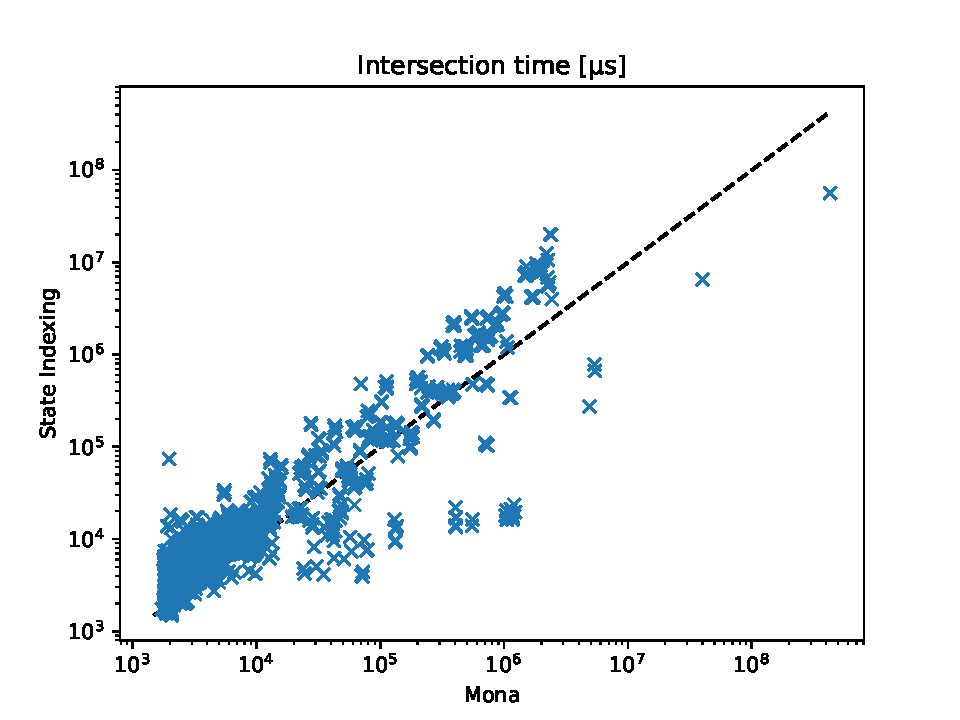
\includegraphics[width=\textwidth]{Figures/intersection-mona.pdf}
                    \caption*{Comparing State Indexing and Mona:\\ Logarithmic Time Performance [$\mu s$].}
                \end{subfigure}
                \begin{subfigure}{0.49\textwidth}
                    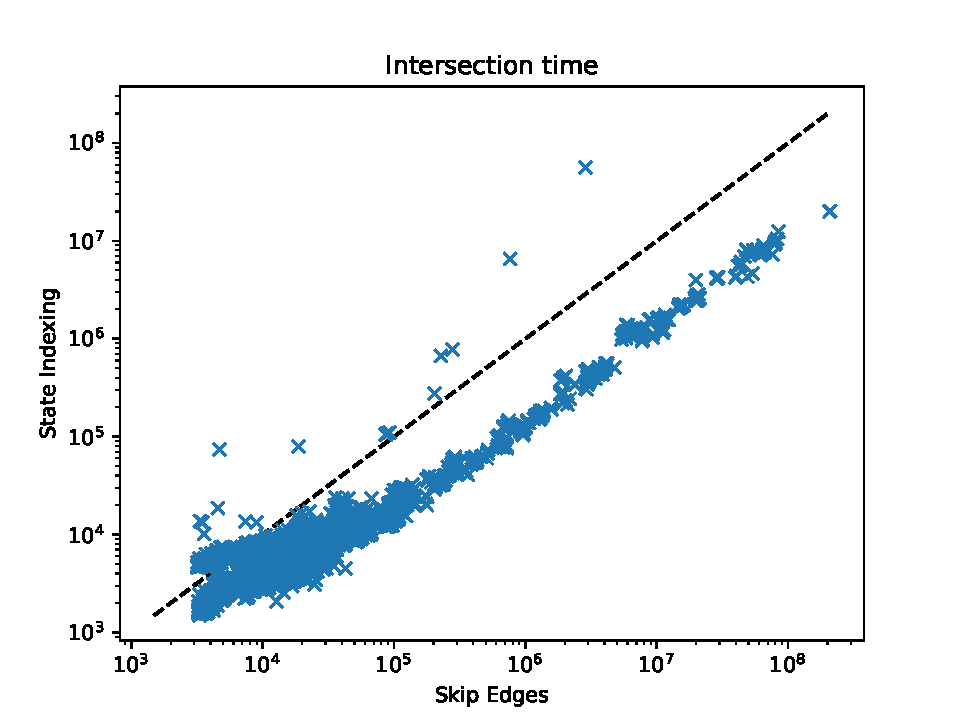
\includegraphics[width=\textwidth]{Figures/intersection-mata.pdf}
                    \subcaption*{Comparing State Indexing and Skip Edges:\\ Logarithmic Time Performance [$\mu s$].}
                \end{subfigure}
                \caption{Comparison of intersection time for the tool Mona, reimplementation using Skip Edges, and reimplementation using State Indexing.}
                \label{fig:intersection_log}
            \end{figure}
            \vspace*{-3em}
            \begin{figure}[h!]
                \centering
                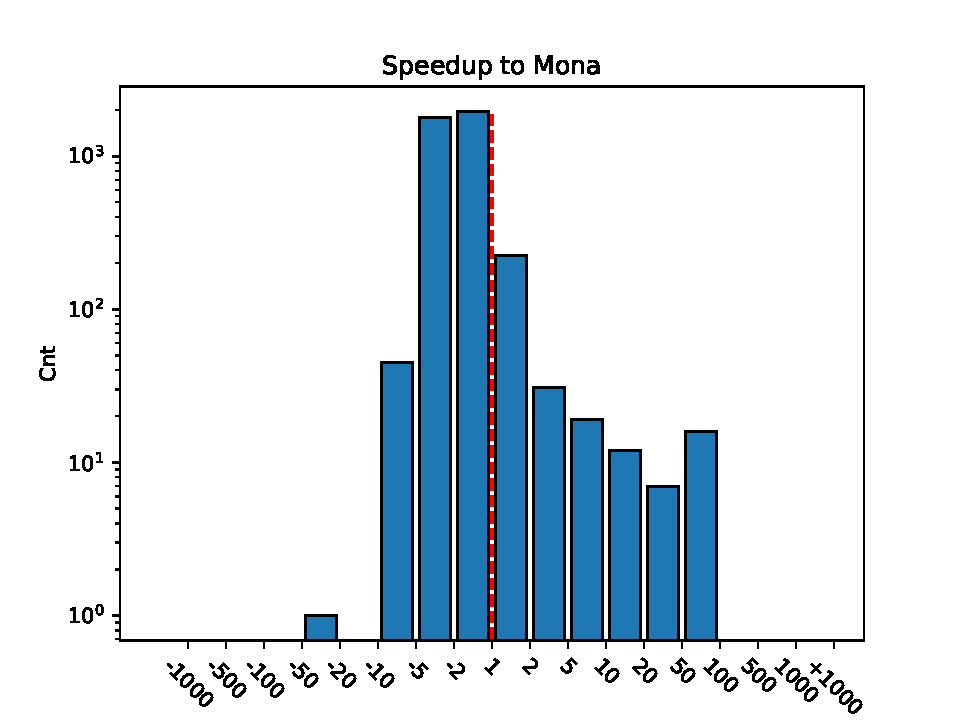
\includegraphics[width=0.49\textwidth]{Figures/intersection-speedup.pdf}
                \caption{State Indexing speedup compared to Mona intersection time. The vertical axis represents the number of occurrences (Logarithmic scale), while the horizontal axis indicates the speedup (positive) or slowdown (negative).}
                \label{fig:intersection_speedup}
            \end{figure}

        \subsubsection*{Projection of the last variable}
            It is interesting to observe, as depicted in Figures \ref{figure:projection_last} and \ref{figure:projection_last_speedup}, that the reimplementation with State Indexing was, on average, faster not only than the Skip Edges version but also than Mona. For certain inputs, State Indexing proved to be more than a thousand times faster than the tool Mona. Despite this, the maximal slowdown for State Indexing was only a factor of 5.
            \begin{figure}[h!]
                \centering
                \captionsetup[subfigure]{justification=centering}
                \begin{subfigure}{0.49\textwidth}
                    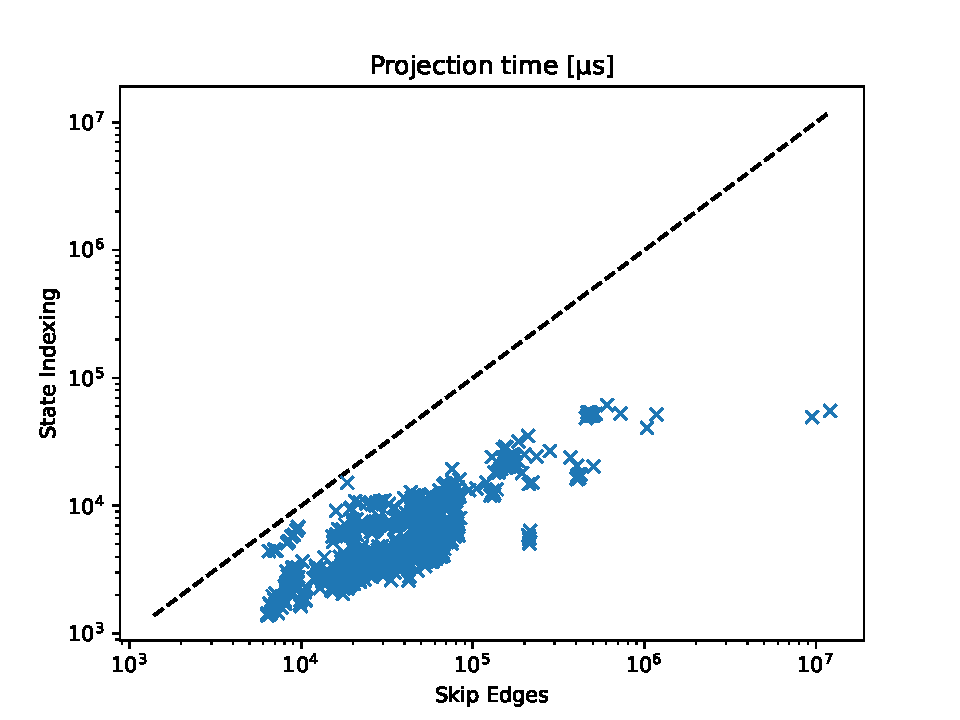
\includegraphics[width=\textwidth]{Figures/projection-last-mata.pdf}
                    \subcaption*{Comparing State Indexing and Mona:\\ Logarithmic Time Performance [$\mu s$].}
                \end{subfigure}
                \begin{subfigure}{0.49\textwidth}
                    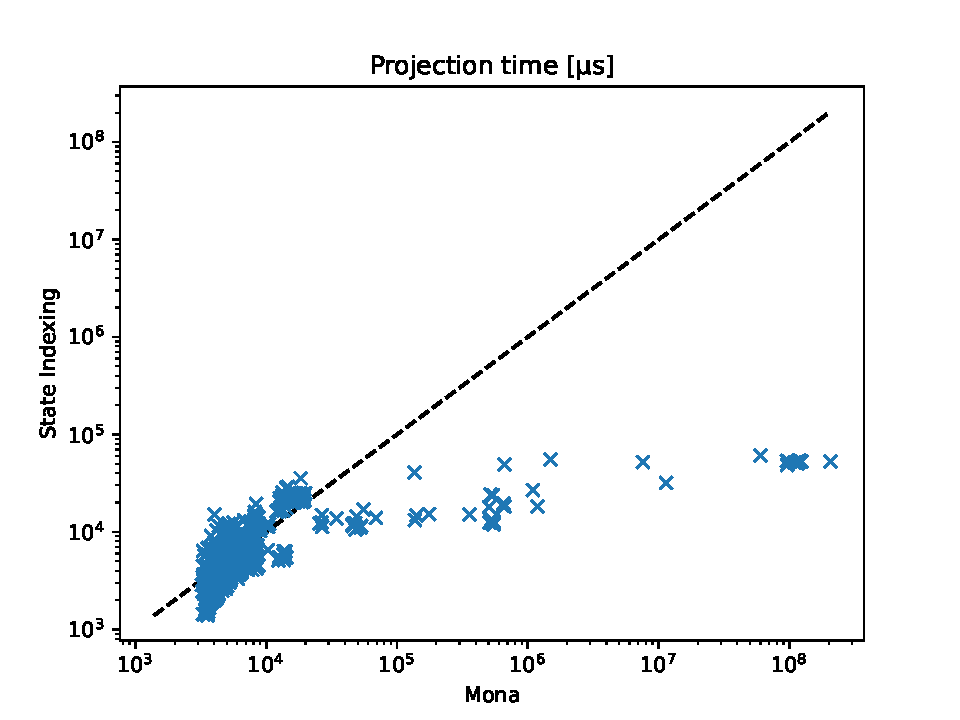
\includegraphics[width=\textwidth]{Figures/projection-last-mona.pdf}
                    \subcaption*{Comparing State Indexing and Skip Edges:\\ Logarithmic Time Performance [$\mu s$].}
                \end{subfigure}
                \caption{Comparison of projection and determinization time for the tool Mona, reimplementation using Skip Edges, and reimplementation using State Indexing.}
                \label{figure:projection_last}
            \end{figure}
            \begin{figure}[h!]
                \centering
                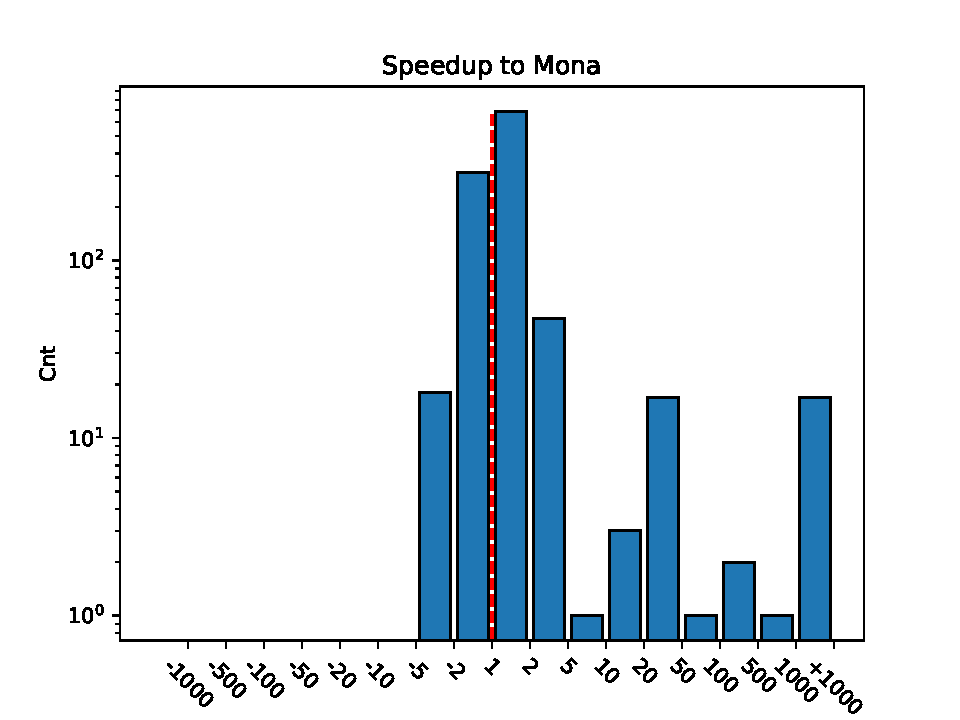
\includegraphics[width=0.49\textwidth]{Figures/projection-last-speedup.pdf}
                \caption{State Indexing speedup compared to Mona projection time. The vertical axis represents the number of occurrences (Logarithmic scale), while the horizontal axis indicates the speedup (positive) or slowdown (negative).}
                \label{figure:projection_last_speedup}
            \end{figure}
        \subsubsection*{Projection of the first variable}
            The projection of the first variable (the variable with the lowest id) was included in the experiments because projecting such a variable yields an automaton with the highest level of nondeterminism, and determinization is performed after every projection. Consequently, it can effectively substitute experiments focused on determinization.

            Unsurprisingly, the State Indexing reimplementation is about ten times faster than Skip Edges. However, it is noteworthy that Mona and State Indexing performed almost identically. This similarity might be due to a less optimized projection algorithm in the Mona tool for the first variable or a potentially suboptimal determinization algorithm.

            \newpage

            \begin{figure}[h!]
                \centering
                \captionsetup[subfigure]{justification=centering}
                \begin{subfigure}{0.49\textwidth}
                    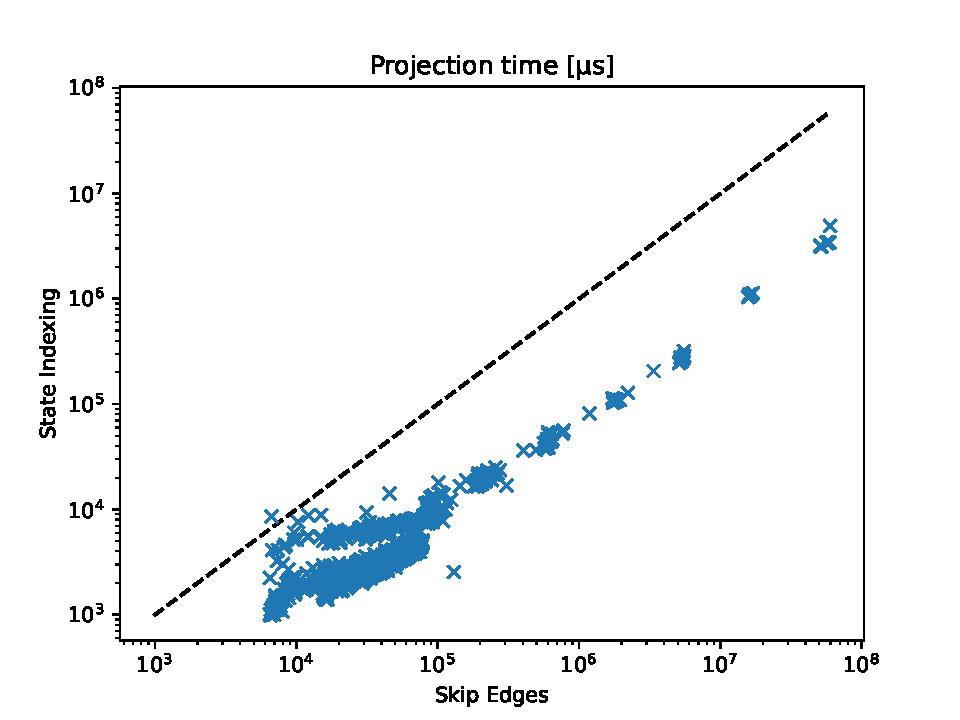
\includegraphics[width=\textwidth]{Figures/projection-first-mata.pdf}
                    \subcaption*{Comparing State Indexing and Mona:\\ Logarithmic Time Performance [$\mu s$].}
                \end{subfigure}
                \begin{subfigure}{0.49\textwidth}
                    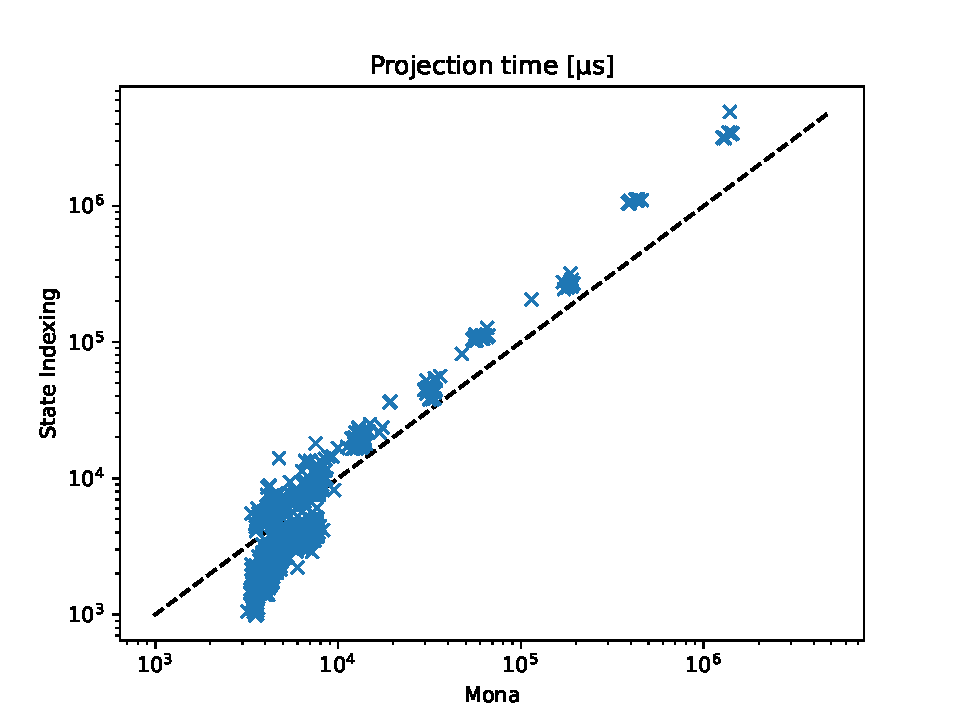
\includegraphics[width=\textwidth]{Figures/projection-first-mona.pdf}
                    \subcaption*{Comparing State Indexing and Skip Edges:\\ Logarithmic Time Performance [$\mu s$].}
                \end{subfigure}
                \label{figure:projection_first}
                \caption{Comparison of projection and determinization time for the tool Mona, reimplementation using Skip Edges, and reimplementation using State Indexing.}
            \end{figure}

            \vspace*{-3em}

            \begin{figure}[h!]
                \centering
                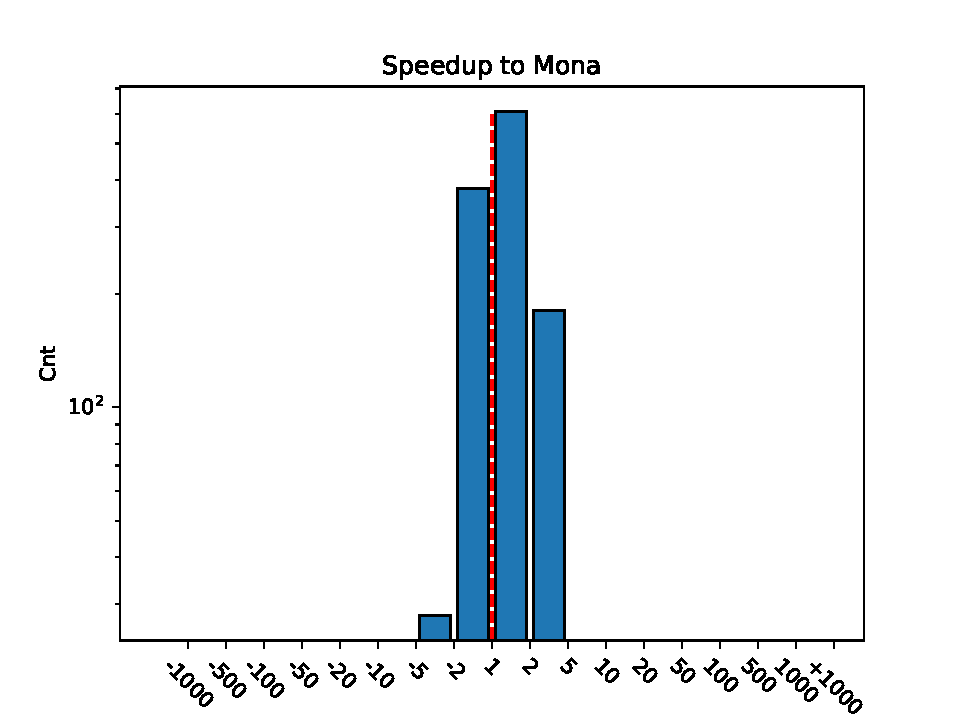
\includegraphics[width=0.49\textwidth]{Figures/projection-first-speedup.pdf}
                \caption{State Indexing speedup compared to Mona projection time. The vertical axis represents the number of occurrences (Logarithmic scale), while the horizontal axis indicates the speedup (positive) or slowdown (negative).}
                \label{figure:projection_first_speedup}
            \end{figure}

    \vspace*{-2em}

    \subsection{WS1S formulae}
        This subsection presents the results of experiments performed on a set of parametric families of WS1S formulae. The first benchmark, \texttt{horn-in}, consists of formulae used to evaluate the Toss tool, as presented in \cite{TOSS}. The second set of families (\texttt{horn-leq}) comes from the work of D'Antoni et al. \cite{DAntoni}, artificially enhanced by added quantifier alternations. The last set of benchmarks (\texttt{horn-trans}, \texttt{set-closed}, and \texttt{set-singletons}) is from the dWiNA tool \cite{dWiNA}.

        \begin{table}[!h]
            \centering
            \captionsetup{width=\textwidth, justification=justified}
            \small
            \begin{tabular}{|l||r|r|r|}
                \hline
                Benchmark        	& SE--Mona [ms] & SI--Mona [ms] & Mona [ms]\\[0.5ex]
                \hline\hline
                \texttt{horn-in}   & $\infty(7)$  & $\infty(6)$ & \cellcolor{gray!25}$\mathbf{\infty(16)}$ \\[0.5ex]
                \texttt{horn-leq}   & 209  & \cellcolor{gray!25}\textbf{101} & $\infty(18)$ \\[0.5ex]
                \texttt{horn-leq $(+3)$}   & 198  & \cellcolor{gray!25}\textbf{88} & $\infty(18)$ \\[0.5ex]
                \texttt{horn-leq $(+4)$}   & 193  & \cellcolor{gray!25}\textbf{88} & $\infty(18)$ \\[0.5ex]
                \texttt{horn-trans}   & $\infty(15)$  & \cellcolor{gray!25}$\mathbf{\infty(20)}$ & $\infty(16)$ \\[0.5ex]
                \texttt{set-closed}   & \cellcolor{gray!25}$\mathbf{\infty(5)}$  & $\infty(4)$ & \cellcolor{gray!25}$\mathbf{\infty(5)}$ \\[0.5ex]
                \texttt{set-singletons}   & $\infty(4)$  & $\infty(4)$ & \cellcolor{gray!25}$\mathbf{\infty(5)}$ \\[0.5ex]

                \hline
            \end{tabular}
            \normalsize
            \vspace*{0.5em}
            \caption{Results for parametrized benchmarks are presented up to $k = 20$. SE--Mona represents a Mona reimplementation using Skip Edges, while SI--Mona stands for the reimplementation utilizing State Indexing. $\infty(n)$ indicates that the cumulative time for the computation of formulae $\leq n$ exceeded the 10-second limit.}
            \label{table}
        \end{table}

        The experiments were focused on the cumulative time of computing parametrized formulae from the easiest to the most difficult. Once the cumulative time exceeded the limit during the computation of the $n$-th formula, the tool was stopped with the result $\infty(n)$. Otherwise, the result was the value of the cumulative time.

        Surprisingly, Mona completely failed on the \texttt{horn-leq} benchmarks. Mona consumed more than ten seconds, while both of its reimplementations, which use DFAs instead of BDDs, finished within 200 milliseconds.

        On the other hand, Mona outperformed both re-implementations on \texttt{horn-in} benchmarks. This could be caused by using an inefficient minimization algorithm (Brzozowski), as on these benchmarks, minimization takes up 98\% of the computation time.

        As expected, the State Indexing reimplementation was faster than Skip Edges and Mona in the majority of benchmarks. However, the speedup was not as significant as one might expect based on the performance of reimplemented automata operations. This behavior is caused by the high number of performed minimizations, which utilizes Brzozowski algorithm.

\section{Conclusion}
    This paper introduces a new reimplementation of the Mona tool for decision procedures in WS1S. The primary motivation was to introduce a pure automata-based approach instead of the combination of BDDs and automata. The reimplementation is based on the master's thesis of Bc. Pavel Bednář, where jumping edges were used to mimic the behavior of BDDs employed by Mona. Our reimplementation utilizes state indexing with the Mata automata library to simulate indexes of inner nodes in BDDs.

    Using the pure automata-based approach, the state indexing method resulted in a~tenfold faster computation of determinization, intersection, and projection. On benchmark formulae designed to stress-test Mona, both reimplementations performed better, with only one exception that can be attributed to using an inefficient Brzozowski minimization algorithm. Our reimplementation outperformed Bednář's approach on the majority of benchmarks, achieving a speedup ranging from two to ten.

    The work can be further improved by implementing a better simulation-based minimization, utilizing abstraction, or by performing operations on nondeterministic finite automata instead of deterministic ones.

    \vspace*{5em}

% \begin{appendices}

% \section{Section title of first appendix}\label{secA1}

% An appendix contains supplementary information that is not an essential part of the text itself but which may be helpful in providing a more comprehensive understanding of the research problem or it is information that is too cumbersome to be included in the body of the paper.

% %%=============================================%%
% %% For submissions to Nature Portfolio Journals %%
% %% please use the heading ``Extended Data''.   %%
% %%=============================================%%

% %%=============================================================%%
% %% Sample for another appendix section			       %%
% %%=============================================================%%

% %% \section{Example of another appendix section}\label{secA2}%
% %% Appendices may be used for helpful, supporting or essential material that would otherwise
% %% clutter, break up or be distracting to the text. Appendices can consist of sections, figures,
% %% tables and equations etc.

% \end{appendices}

%%===========================================================================================%%
%% If you are submitting to one of the Nature Portfolio journals, using the eJP submission   %%
%% system, please include the references within the manuscript file itself. You may do this  %%
%% by copying the reference list from your .bbl file, paste it into the main manuscript .tex %%
%% file, and delete the associated \verb+\bibliography+ commands.                            %%
%%===========================================================================================%%

\bibliography{sn-bibliography}% common bib file
%% if required, the content of .bbl file can be included here once bbl is generated
%%\input sn-article.bbl


\end{document}
